Niezależnie od tego czy posiadasz płytę główną z BIOSem czy z UEFI, w poprzednim punkcie powinieneś wybrać "Zainstaluj Ubuntu". Ta metoda jest szybsza od "Wypróbuj Ubuntu bez instalowania" gdyż nie wymaga załadowania całego systemu. Jeżeli mimo wszystko uruchomiłeś cały system, to na jego pulpicie znajdziesz ikonę "Zainstaluj Ubuntu" (lub "Install Ubuntu", jeżeli nie zmieniałeś języka). Od tego momentu instalacja przebiega w identyczny sposób dla każdego wybranego sposobu instalacji.
W czasie instalacji, w prawej część paska u góry ekranu znajduje się szerego ikon:
\begin{description}
\item[
\includegraphics{images/ikony_dostempnosc.png}]Dostępność - uruchomienie lupy, czytnika ekranowego lub klawiatury ekranowej.
\item[
\includegraphics{images/ikony_internet.png}]Łączność - pozwala skonfigurować połączenie z internetem na czas instalacji systemu.
\item[
\includegraphics{images/ikony_jezyk.png}]Język - pozwala zmienić język oraz ukłąd klawiatury na czas instalacji systemu.
\item[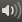
\includegraphics{images/ikony_dzwiek.png}]Ustawienia głośności i dźwięku
\item[
\includegraphics{images/ikony_zasilanie.png}]Wyłączenie lub ponowne uruchomienie komputera.
\end{description}
\clearpage
\subsubsection{Wybór języka}
\begin{center}
        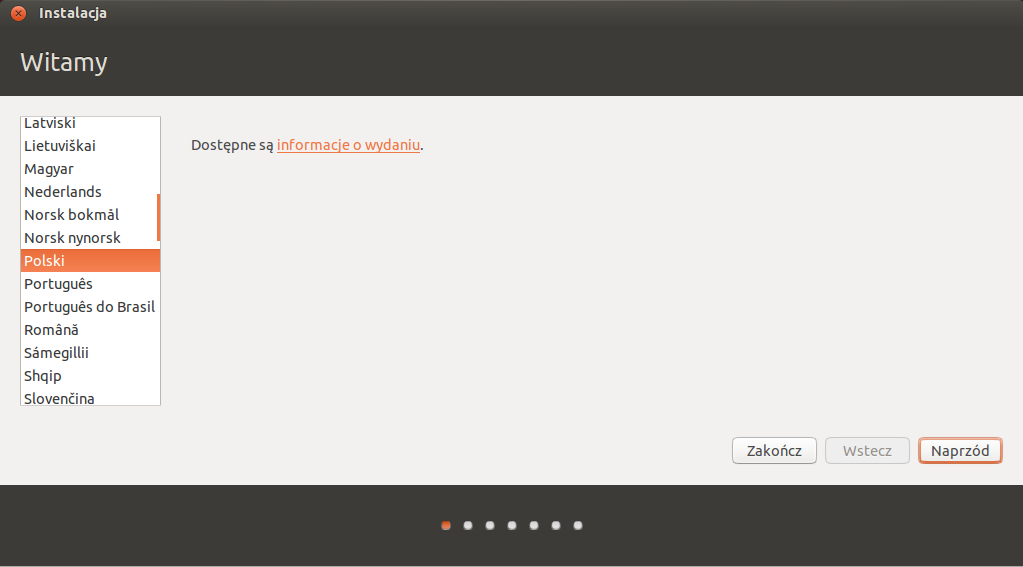
\includegraphics[scale=0.5]{images/instalator_jezyk.png}]
\end{center}
Pierwszy ekran instalatora pozwala wybrać język. Jeżeli wcześniej nie zmieniłeś języka na Polski to teraz masz ku temu okazję. Język wybrany podczas instalacji będzie także domyślnym językiem zainstalowanym w systemie.
\begin{flushright}
Kliknij na przycisk \textbf{Naprzód} aby przejść dalej.
\end{flushright}
\clearpage
\subsubsection{Konfiguracja WiFi}
Do opisania
%TODO
\clearpage
\subsubsection{Sprawdzenie kompatybilności sprzętu, wybór dodatkowych komponentów}
\begin{center}
        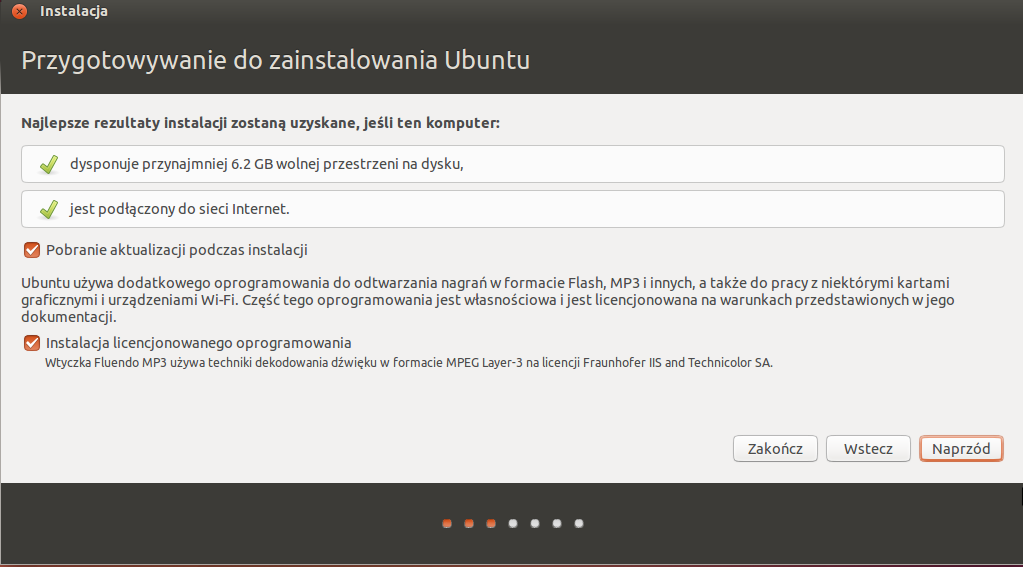
\includegraphics[scale=0.5]{images/instalator_wymagania.png}]
\end{center}
Na tym etapie instalator sprawdzi, czy na dysku twardym jest wystarczająco miejsca aby zainstalować Ubuntu. Połączenie z internetem nie jest wymagane aby zainstalować system. Połączenie z internetem jest niezbędne aby zainstalować spolszczenie systemu, aktualizacje oraz dodatkowe wtyczki. Jeżeli w tym momęcie nie masz połączenia z internetem to pobranie paczek lokalizacyjnych będzie możliwe później. Zostało to opisane w rozdziale \ref{sec:rzeczy_do_zrobienia_po_instalacji} "Rzeczy do zrobienia po instalacji Ubuntu".
\begin{description}
\item[Pobieranie aktualizacji podczas instalacji] - Instalator pobierze i zainstaluje wszystkie aktualizacje, które zostały wydane od dnia premiery systemu.
\item[Instalacja licencjonowanego oprogramowania] - W skład pakietu wchodzą własnościowe sterowniki dla kart graficznych AMD oraz Nvidia, sterowniki dla kart Wi-Fi, kodeki audio-wideo (po instalacji Ubuntu będzie wstanie obsłużyć prawie każdy rodzaj muzyki i filmów) oraz wtyczka flash do przeglądarki internetowej.
\end{description}
\begin{flushright}
Kliknij na przycisk \textbf{Naprzód} aby przejść dalej.
\end{flushright}
\clearpage
\subsubsection{Partycjonowanie dysku twardego}
\begin{center}
        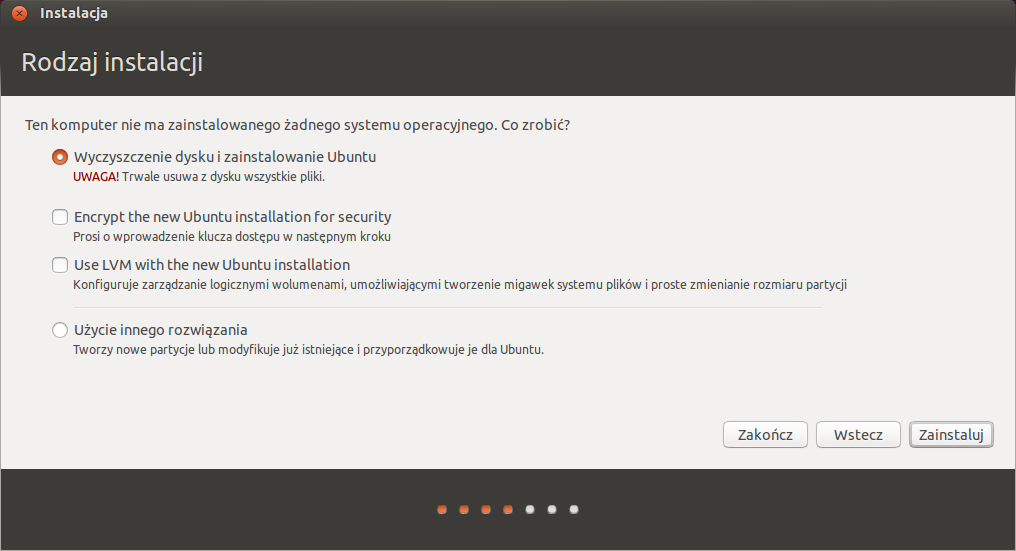
\includegraphics[scale=0.5]{images/instalator_partycjonowanie_proste.png}]
\end{center}
Jest to najważniejszy etap instalacji. W tym miejscu można dokonać cudów jak i zniszczyć cały dysk twardy. Jako, że prawidłowe partycjonowanie dysku twardego to bardzo szeroki temat to poświęciliśmy mu cały osobny rozdział. Na powyższym obrazie widać najprostszą wersję tego etapu instalacji. Na dysku twardym nie ma zainstalowanego żadnego systemu operacyjnego i instalator proponuje wykorzystanie całej przestrzeni dla Ubuntu. Jeżeli masz inne systemy operacyjne to instalator zaproponuje wydzielenie miejsca i instalację Ubuntu obok danego systemu operacyjnego. Jeżeli miałeś wcześniej zainstalowane Ubuntu, instalator zaproponuje aktualizację do najnowszego wydania lub usunięcie i zainstalowanie Ubuntu ponownie.
Partycjonowanie zostało szeroko opisane w rozdziale \ref{subsec:partycjonowanie} "Zaawansowane partycjonowanie". Wróć tutaj jak go przeczytasz.
\begin{flushright}
Kliknij na przycisk \textbf{Naprzód} aby przejść dalej.
\end{flushright}
\clearpage
\subsubsection{Wybór strefy czasowej}
\label{subsub:instalator_strefa_czasowa}
\begin{center}
        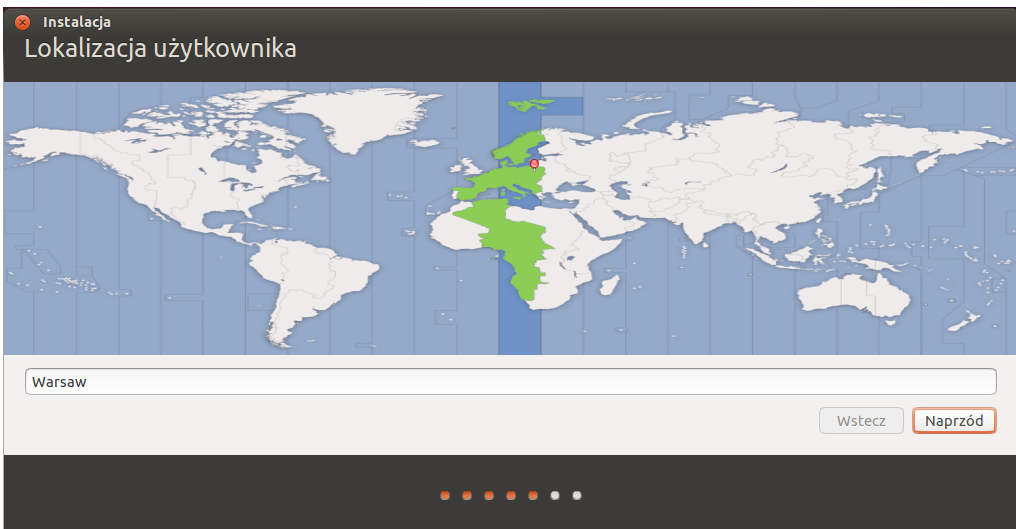
\includegraphics[scale=0.5]{images/instalator_czas.png}]
\end{center}
Na tym etapie należy wybrać lokalizację tego komputera, tak aby system mógł wyświetlać prawidłowy czas i automatycznie dostosowywać się do zmian pomiędzy czasem letnim i zimowym. Jeżeli w trakcie instalacji masz połączenie z internetem to odpowiednia lokalizacja zostanie sama wybrana. Jeżeli nie masz dostępu do internetu w pole wpisz "Warsaw". Stolica naszego kraju określa też nasza strefę czasową.
\begin{flushright}
Kliknij na przycisk \textbf{Naprzód} aby przejść dalej.
\end{flushright}
\clearpage
\subsubsection{Wybór układu klawiatury}
\begin{center}
        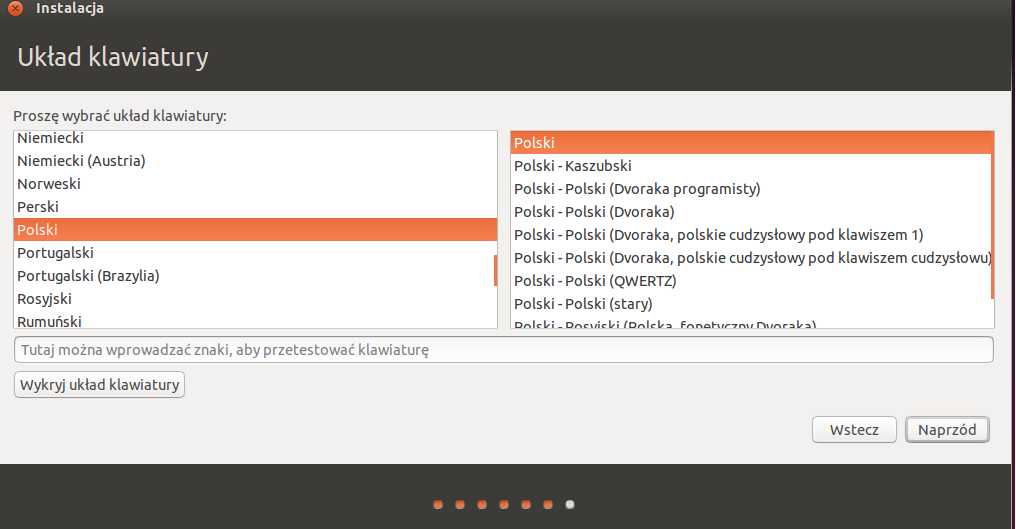
\includegraphics[scale=0.5]{images/instalator_klawiatura.png}]
\end{center}
Ten ekran pozwala wybrać układ klawiatury. Jeżeli wybrałeś wcześniej język Polski, to standardowa polska klawiatura zostanie tutaj automatycznie wybrana. W polu możesz wpisać kilka znaków aby sprawdzić czy zaznaczony układ odpowiada rzeczywistości. Pierwsza opcja ("Polski") to standardowa klawiatura 101 klawiszy, zwana potocznie układem programisty.
Nie zalecamy korzystania z funkcji "Wykryj układ klawiatury". Korzystając ze wskazówek instalatora otrzymamy klawiaturę amerykańską, nie obsługującą polskich znaków diakrytycznych.
\begin{flushright}
Kliknij na przycisk \textbf{Naprzód} aby przejść dalej.
\end{flushright}
\clearpage
\subsubsection{Toższamość użytkownika}
\begin{center}
        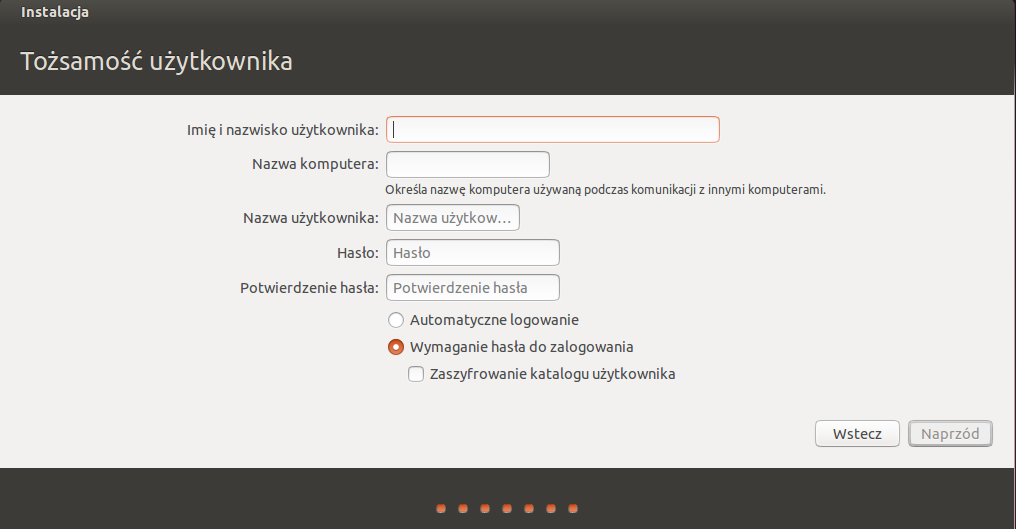
\includegraphics[scale=0.5]{images/instalator_dane.png}]
\end{center}
To już ostatni etap instalacji. Te pola należy uzupełnić aby system mógł cię prawidłowo zidentyfikować.
\begin{description}
\item[Imię i nazwisko użytkownika] - Pole nieobowiązkowe, ale jeżeli uzupełnisz te dane to system będzie się do ciebie zwracał z imienia i nazwiska zamiast używać loginu (np. Jan Kowalski).
\item[Nazwa komputera] - Określa jak będzie się nazywał twój komputer (np. laptop).
\item[Nazwa użytkownika] - Twój login do systemu (np. jan\_kowalski albo twój pseudonim). Login nie może zawierać dużych liter, spacji ani znaków specjalnych.
\item[Hasło] - Hasło do komputera. Hasło zabezpiecza system przed nieuprawnionym dostępem. Uwaga: Ustawienie hasła uniemożliwia innym zalogowanie się do twojego konta, jednak nie zabezpiecza innych przed podglądem twoich dany o ile ich nie zaszyfrujesz. 
\item[Potwierdzenie hasła] - Wpisz ponownie to samo hasło co w polu powyżej.
\item[Automatyczne logowanie] - Jeżeli zaznaczysz to pole, to system automatycznie zaloguje tego użytkownika po uruchomieniu. Nie będzie potrzebne podawanie hasła aby uzyskać dostęp do komputera.
\item[Wymaganie hasła do zalogowania] - Po uruchomieniu komputera będziesz musiał podać hasło aby uzyskać dostęp do swojego konta.
\item[Zaszyfrowanie katalogu użytkownika] - Jeżeli zaznaczysz to pole to twoje prywatne dane zostaną zaszyfrowane. Nikt nie znający hasła nie będzie mógł uzyskać dostępu do twoich plików. Jeżeli zapomnisz hasła to bezpowrotnie utracisz dostęp do swoich plików.
\end{description}
\begin{flushright}
Kliknij na przycisk \textbf{Naprzód} aby przejść dalej.
\end{flushright}
\clearpage
\subsubsection{Instalacja}
\begin{center}
        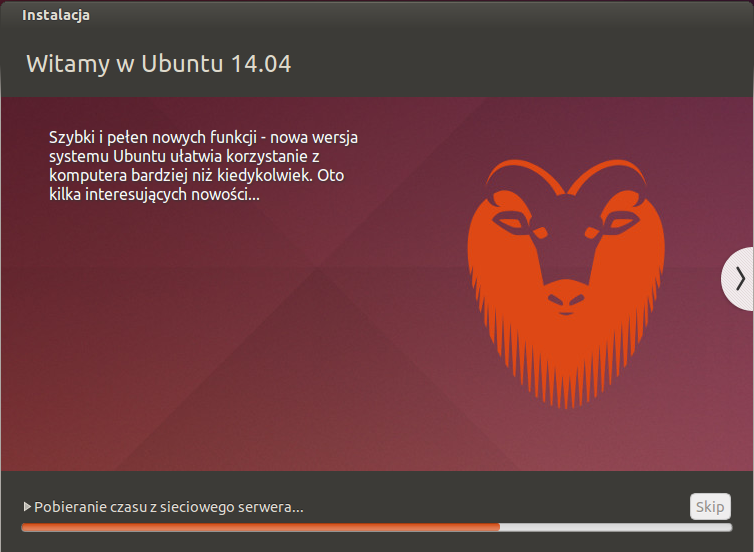
\includegraphics[scale=0.5]{images/instalator_kopiowanie.png}]
\end{center}
Teraz system dokona instalacji na dysku twardym i ewentualnie pobierze i zainstaluje paczki językowe, aktualizacje i dodatkowe oprogramowanie. Proces ten może potrwać od kilku do kilkunastu minut w zależności od klasy komputera, ilości zadań do wykonania oraz szybkości łącza internetowego.
Po zakończeniu instalacji zostaniesz poproszony o usunięcie nośnika instalacyjnego i ponowne uruchomienie komputera. Jeżeli wszystko poszło pomyślnie to za minutę zostaniesz przywitanym pulpitem Ubuntu.
\begin{flushright}
\textbf{Gratulacje!} Właśnie zainstalowałeś Ubuntu 14.04 LTS Trusty Thar.\\
Komputer zostanie zresetowany.\\
Przejdź do sekcji \ref{sec:pierwsze_uruchomienie}:"Pierwsze Uruchomienie Ubuntu"
\end{flushright}
\clearpage
